\makesectionpage[figures/quiz.png]{Modellauswahl}

\makesubsectionpage{Score berechnen}

\begin{frame}{Train/Test und Verallgemeinerung}
\begin{columns}
\column{0.6\textwidth}
\begin{itemize}
    \item Trainingsdaten decken meist nur einen Teil möglicher Eingaben ab
    \item Modell muss auch für unbekannte Eingaben sinnvolle Ergebnisse liefern
    \item Diese Fähigkeit heißt \textbf{Verallgemeinerung}
    \item Verallgemeinerungsfähigkeit ist zentrales Qualitätsmaß
    \item Bewertung nur mit \textbf{unbekannten Testdaten}
    \item Typische Aufteilung:
    \begin{itemize}
    \item \textbf{75\%} Training
    \item \textbf{25\%} Test
\end{itemize}
\end{itemize}

\column{0.35\textwidth}
\twemoji[width=0.9\linewidth]{cake}

\end{columns}
\source{\cite{seemann2024mlaz}}
\end{frame}



\begin{frame}{Train/Test}

\begin{columns}
\begin{column}{0.35\textwidth}

\textbf{Nach welchem Kriterium soll man aufteilen?} 

In der Praxis hat sich die \emph{einfache zufällige Aufteilung} (Random Split) bewährt. Dabei werden die Beobachtungen nach dem Zufallsprinzip in Trainings- und Testdaten aufgeteilt.
\end{column}


\begin{column}{0.6\textwidth}
\centering

\begin{tikzpicture}[
    x=0.045cm,
    y=0.0028cm,
    >=latex,
    font=\scriptsize,
    scale=1.2
]

    % Hintergrund
    \fill[BlockBackground] (0,0) rectangle (140,1600);

    % Horizontale Gitterlinien
    \foreach \yy in {200,400,...,1600}{
        \draw[DarkGrey!60, line width=0.4pt]
            (0,\yy) -- (140,\yy);
    }

    % Achsen
    \draw[TextColor, line width=1pt, ->] (0,0) -- (146,0);
    \draw[TextColor, line width=1pt, ->] (0,0) -- (0,1700);

    % x-Ticks
    \foreach \xx in {0,20,...,140}{
        \draw[TextColor] (\xx,0) -- (\xx,-35);
        \node[anchor=north,text=DarkGrey] at (\xx,-40) {\tiny \xx};
    }

    % y-Ticks
    \foreach \yy in {0,200,...,1600}{
        \draw[TextColor] (0,\yy) -- (-3,\yy);
        \node[anchor=east,text=DarkGrey] at (-4,\yy) {\tiny \yy};
    }

    % Achsenbeschriftungen
    \node[
        rotate=90,
        align=center,
        text=TextColor,
        font=\scriptsize\bfseries
    ] at (-19,800) {Monatsmiete in €};

    \node[
        align=center,
        text=TextColor,
        font=\scriptsize\bfseries
    ] at (70,-190) {Wohnungsgröße in qm};

 

    % Messpunkte
    \foreach \x/\y in {
        10/140,
        27/250,
        50/660,
        64/530,
        80/800,
        85/1020,
        95/1010,
        115/1200,
        120/1520
    }{
        \filldraw[
            fill=AccentColor,
            draw=AccentTitle,
            line width=0.8pt
        ] (\x,\y) circle (3pt);
    }

       % Regressionsgerade
    \draw[
        PrimaryColor,
        line width=1.5pt
    ] (0,0) -- (140,1600);

\end{tikzpicture}

\end{column}
\end{columns}
\note{Die lineare Regression ist unser erstes Machine Learning Modell.\\
Auf Basis der Größe einer Wohnung möchten wir vorhersagen, welche Miete wir erzielen können.
}
\source{\cite{seemann2024mlaz}}
\end{frame}


\begin{frame}[fragile]{Train/Test in Python}
\footnotesize
\begin{columns}
\column{0.35\textwidth}
\begin{itemize}
    \item Funktion \texttt{train\_test\_split()} teilt Datenmenge auf
    \item Übergabe von Eingabe- (\texttt{X}) und Zielwerten (\texttt{Y})
    \item Aufteilung erfolgt gemäß Parameter
    \item Rückgabe von \textbf{vier Datensätzen}:
    \begin{itemize}
        \item \texttt{X\_train}, \texttt{X\_test}
        \item \texttt{Y\_train}, \texttt{Y\_test}
    \end{itemize}
    
    \item \texttt{random\_state} ist \textbf{optional}
    
\end{itemize}

\column{0.60\textwidth}
\begin{minted}[fontsize=\footnotesize]{python}
from sklearn.model_selection import train_test_split

X = df[["Quadratmeter"]].to_numpy()
Y = df[["Kaltmiete"]].to_numpy()

X_train, X_test, y_train, Y_test = train_test_split(
    X, Y,
    random_state=0
)
\end{minted}
\end{columns}
\source{\cite{seemann2024mlaz}, RegressionMieten.ipynb}
\end{frame}


\begin{frame}{Bewertung von Regressionsmodellen}
\begin{columns}
\column{0.48\textwidth}
\includesvg[width=\linewidth]{figures/regression_plot}

\column{0.47\textwidth}
\begin{itemize}
    \item In der letzten Übung: Modell zur Vorhersage des \textbf{Fahrzeugverbrauchs}
    \item \textbf{Eingabe: } Gewicht des Fahrzeugs
    \item \textbf{Ziel: } Verbrauch abschätzen
    \item \textbf{Beobachtung: }
    \begin{itemize}
        \item Reale Datenpunkte weichen teilweise deutlich ab
        \item Modell trifft nicht immer exakte Vorhersagen
    \end{itemize}
    \item \textbf{Frage: }Wie gut ist das Modell wirklich?
\end{itemize}
\end{columns}
\source{\cite{seemann2024mlaz}, LösungRegressionMpg.ipynb}
\end{frame}

\begin{frame}{Bewertung von Regressionsmodellen}
    
\begin{columns}
\column{0.7\textwidth}
\begin{itemize}
    \item Vermutlich lässt sich das Modell \textbf{verbessern}
    \item Wir könnten \textbf{zusätzliche Merkmale} in die Vorhersage einbeziehen
\end{itemize}

\vspace{0.4em}

\scriptsize
\begin{tabular}{lrrrrrrrrl}
\textbf{mpg} & \textbf{cyl} & \textbf{disp} & \textbf{hp} & \textbf{weight} & \textbf{acc} & \textbf{year} & \textbf{org} & \textbf{name}\\
18.0 & 8 & 307.0 & 130 & 3504 & 12.0 & 70 & 1 & chevrolet ...  \\
15.0 & 8 & 350.0 & 165 & 3693 & 11.5 & 70 & 1 & buick ... \\
18.0 & 8 & 318.0 & 150 & 3436 & 11.0 & 70 & 1 & plymouth ... \\
16.0 & 8 & 304.0 & 150 & 3433 & 12.0 & 70 & 1 & amc ... \\
17.0 & 8 & 302.0 & 140 & 3449 & 10.5 & 70 & 1 & ford ... \\
\end{tabular}

\column{0.3\textwidth}
\begin{block}{Hinweis}
Zum Vergleich von Modellen benötigt man ein Maß für die Prognosegüte.

Dies liefert das \textbf{Bestimmtheitsmaß} $R^2$.
\end{block}
\end{columns}
\end{frame}

\begin{frame}{Bestimmtheitsmaß}
\begin{columns}
\column{0.35\textwidth}
\textbf{Grundidee:}
\begin{itemize}
    \item Vergleich mit einfachem Modell
    \item Dieses gibt immer den \textbf{Mittelwert} der Zielwerte zurück
    \item Vergleich:
    \begin{itemize}
        \item \textbf{Quadratischer Fehler} des Modells
        \item vs. Fehler des \textbf{Vergleichsmodells}
    \end{itemize}
\end{itemize}

\column{0.6\textwidth}
\centering
\begin{tikzpicture}[
    x=0.045cm,
    y=0.0028cm,
    >=latex,
    font=\scriptsize,
    scale=1.1
]

    % Hintergrund
    \fill[BlockBackground] (0,0) rectangle (140,1600);

    % Horizontale Gitterlinien
    \foreach \yy in {200,400,...,1600}{
        \draw[DarkGrey!60, line width=0.4pt]
            (0,\yy) -- (140,\yy);
    }

    % Achsen
    \draw[TextColor, line width=1pt, ->] (0,0) -- (146,0);
    \draw[TextColor, line width=1pt, ->] (0,0) -- (0,1700);

    % x-Ticks
    \foreach \xx in {0,20,...,140}{
        \draw[TextColor] (\xx,0) -- (\xx,-35);
        \node[anchor=north,text=DarkGrey] at (\xx,-40) {\tiny \xx};
    }

    % y-Ticks
    \foreach \yy in {0,200,...,1600}{
        \draw[TextColor] (0,\yy) -- (-3,\yy);
        \node[anchor=east,text=DarkGrey] at (-4,\yy) {\tiny \yy};
    }

    % Beschriftungen
    \node[rotate=90, text=TextColor, font=\scriptsize\bfseries]
        at (-19,810) {Monatsmiete in €};

    \node[text=TextColor, font=\scriptsize\bfseries]
        at (70,-190) {Wohnungsgröße in qm};

    % Punkte
    \foreach \x/\y in {
        10/140,
        27/250,
        50/660,
        64/530,
        80/800,
        85/1020,
        95/1010,
        115/1200,
        120/1520
    }{
        \filldraw[fill=AccentColor, draw=AccentTitle, line width=0.8pt]
            (\x,\y) circle (3pt);
    }

    % Mittelwertlinie
    \draw[PrimaryColor, line width=1.5pt]
        (0,791) -- (140,791);

    \node[text=PrimaryColor, anchor=west]
        at (90,850) {\scriptsize Mittelwert 791€ = $\bar{y}$};

\end{tikzpicture}
\end{columns}
\source{\cite{seemann2024mlaz}}
\end{frame}

\begin{frame}{Bestimmtheitsmaß}
\begin{columns}
\column{0.35\textwidth}
{Quadratischer Fehler des \textbf{Vergleichsmodells}:}
    \[
        E_{\text{vergleich}} 
        = \sum (y_i - \bar{y})^2
    \]

\column{0.6\textwidth}
\centering
\begin{tikzpicture}[
    x=0.045cm,
    y=0.0028cm,
    >=latex,
    font=\scriptsize,
    scale=1.1
]

    % Hintergrund
    \fill[BlockBackground] (0,0) rectangle (140,1600);

    % Gitter
    \foreach \yy in {200,400,...,1600}{
        \draw[DarkGrey!60, line width=0.4pt]
            (0,\yy) -- (140,\yy);
    }

    % Achsen
    \draw[TextColor, line width=1pt, ->] (0,0) -- (146,0);
    \draw[TextColor, line width=1pt, ->] (0,0) -- (0,1700);

    % x-Ticks
    \foreach \xx in {0,20,...,140}{
        \draw[TextColor] (\xx,0) -- (\xx,-35);
        \node[anchor=north,text=DarkGrey] at (\xx,-40) {\tiny \xx};
    }

    % y-Ticks
    \foreach \yy in {0,200,...,1600}{
        \draw[TextColor] (0,\yy) -- (-3,\yy);
        \node[anchor=east,text=DarkGrey] at (-4,\yy) {\tiny \yy};
    }

    % Punkte
    \foreach \x/\y in {
        10/140,
        27/250,
        50/660,
        64/530,
        80/800,
        85/1020,
        95/1010,
        115/1200,
        120/1520
    }{
     % vertikale gestrichelte Linie
        \draw[dashed, DarkGrey]
            (\x,\y) -- (\x,791);    
    
    \filldraw[fill=AccentColor, draw=AccentTitle, line width=0.8pt]
            (\x,\y) circle (3pt);

       
    }
   
    % Beschriftungen
    \node[rotate=90, text=TextColor, font=\scriptsize\bfseries]
        at (-19,810) {Monatsmiete in €};

    \node[text=TextColor, font=\scriptsize\bfseries]
        at (70,-190) {Wohnungsgröße in qm};

    % Mittelwertlinie
    \draw[PrimaryColor, line width=1.5pt]
        (0,791) -- (140,791);

    \node[text=PrimaryColor, anchor=west]
        at (130,850) {\scriptsize $\bar{y}$};

    % Beschriftung einer Differenz
    \node[text=TextColor]
        at (75,650) {\scriptsize $y_i - \bar{y}$};

\end{tikzpicture}
\end{columns}
\source{\cite{seemann2024mlaz}}
\end{frame}


\begin{frame}{Bestimmtheitsmaß}
\begin{columns}
\column{0.35\textwidth}
Quadratischer Fehler des \textbf{Regressionsmodells}:
    \[
        E_{\text{modell}} 
        = \sum (y_i - \hat{y}_i)^2
    \]

\column{0.6\textwidth}
\centering
\begin{tikzpicture}[
    x=0.045cm,
    y=0.0028cm,
    >=latex,
    font=\scriptsize,
    scale=1.1
]

    % Hintergrund
    \fill[BlockBackground] (0,0) rectangle (140,1600);

    % Gitter
    \foreach \yy in {200,400,...,1600}{
        \draw[DarkGrey!60, line width=0.4pt]
            (0,\yy) -- (140,\yy);
    }

    % Achsen
    \draw[TextColor, line width=1pt, ->] (0,0) -- (146,0);
    \draw[TextColor, line width=1pt, ->] (0,0) -- (0,1700);

    % x-Ticks
    \foreach \xx in {0,20,...,140}{
        \draw[TextColor] (\xx,0) -- (\xx,-35);
        \node[anchor=north,text=DarkGrey] at (\xx,-40) {\tiny \xx};
    }

    % y-Ticks
    \foreach \yy in {0,200,...,1600}{
        \draw[TextColor] (0,\yy) -- (-3,\yy);
        \node[anchor=east,text=DarkGrey] at (-4,\yy) {\tiny \yy};
    }

    % Achsenbeschriftungen
    \node[rotate=90, text=TextColor, font=\scriptsize\bfseries]
        at (-19,800) {Monatsmiete in €};

    \node[text=TextColor, font=\scriptsize\bfseries]
        at (70,-190) {Wohnungsgröße in qm};

    % Punkte + Abstände zur Regressionsgeraden
    \foreach \x/\y in {
        10/140,
        27/250,
        50/660,
        64/530,
        80/800,
        85/1020,
        95/1010,
        115/1200,
        120/1520
    }{
        % approx. Projektion auf Gerade y = 11.3*x (visuell)
        \pgfmathsetmacro{\yhat}{11.3*\x}

        \draw[dashed, DarkGrey]
            (\x,\y) -- (\x,\yhat);

        \filldraw[fill=AccentColor, draw=AccentTitle, line width=0.8pt]
            (\x,\y) circle (3pt);
    }

    % Regressionsgerade (y-hat)
    \draw[PrimaryColor, line width=1.5pt]
        (0,0) -- (140,1580);

    \node[text=PrimaryColor, anchor=west]
        at (95,1200) {\scriptsize $\hat{y}$};

    % Beschriftung eines Abstands
    \node[text=TextColor]
        at (75,640) {\scriptsize $y_i - \hat{y}_i$};

\end{tikzpicture}
\end{columns}
\source{\cite{seemann2024mlaz}}
\end{frame}


\begin{frame}{Bestimmtheitsmaß}
\begin{columns}
\column{0.47\textwidth}

\begin{blockDef}{Definition Bestimmtheitsmaß}
\[
R^2 \coloneqq 
1 - 
\frac{\sum (y_i - \hat{y}_i)^2}
     {\sum (y_i - \bar{y})^2}
\]

\end{blockDef}

\vspace{0.5em}

\begin{itemize}
    \item Fehler des Vergleichsmodells
    \item relativ zum Fehler des zu bewertenden Modells
\end{itemize}

\column{0.48\textwidth}
\footnotesize
\textbf{Was sagt uns das Bestimmtheitsmaß?}

\begin{itemize}
    \item Perfekte Vorhersage:
    \[
    R^2 = 1 - \frac{0}{E_{\text{vergleich}}} = 1
    \]

    \item Gleich schlecht wie Vergleichsmodell:
    \[
    R^2 = 1 - \frac{E_{\text{modell}}}{E_{\text{vergleich}}}
        = 1 - 1 = 0
    \]

    \item Besser als Vergleichsmodell:
    \begin{itemize}
        \item $0 < R^2 \leq 1$
        \item Je näher an 1, desto besser
    \end{itemize}
\end{itemize}

\end{columns}
\source{\cite{seemann2024mlaz}}
\end{frame}


\begin{frame}[fragile]{Bestimmtheitsmaß: Berechnung in Python}
\begin{columns}
\column{0.35\textwidth}

Berechnung des $R^2$ für das Miles-per-Gallon-Modell. \textbf{Variante 1:}


\vspace{0.3em}

\begin{enumerate}
    \item Modell wie gewohnt trainieren
    \item Prognosen für Testdaten berechnen
    \item $R^2$ mit \texttt{r2\_score} bestimmen
\end{enumerate}

\column{0.60\textwidth}
\begin{minted}[fontsize=\footnotesize]{python}
# Vorhersagen für die Testdaten berechnen
y_test_predicted = model.predict(X_test)

from sklearn.metrics import r2_score
# R^2 berechnen 
r2 = r2_score(Y_test, y_test_predicted)

# Ergebnis ausgeben
print(r2)
\end{minted}

\vspace{0.4em}

\textbf{Ausgabe:}\\
\centering
\texttt{0.6848680875703099}


\end{columns}
\source{BestimmtheitsmaßBerechnen.ipynb}
\end{frame}


\begin{frame}[fragile]{Bestimmtheitsmaß: Berechnung in Python}
\begin{columns}
\column{0.35\textwidth}

\textbf{Variante 2:}

\begin{itemize}
    \item Daten laden und Modell wie gewohnt trainieren
    \item Bestimmtheitsmaß direkt über das Modell berechnen
    \item Verwendung der Methode \texttt{score()}
    \item Kein explizites \texttt{predict()} 
\end{itemize}



\column{0.60\textwidth}

\begin{minted}[fontsize=\footnotesize]{python}
# R^2 direkt über das Modell berechnen
r2 = model.score(X_test, Y_test)

# Ergebnis ausgeben
print(r2)
\end{minted}

\textbf{Ausgabe:}\\
\centering
\texttt{0.6848680875703099}

\end{columns}
\source{BestimmtheitsmaßBerechnen.ipynb}
\end{frame}


\begin{frame}[fragile]{Aufgabe: Modelle vergleichen}
\begin{columns}

\column{0.70\textwidth}
\footnotesize
Wir betrachten wieder die Datei mit dem Spritverbrauch  \texttt{auto-mpg.csv}.

\textbf{Aufgaben:}
\begin{itemize}
\item Erweitern Sie Ihr Notebook, sodass das Bestimmtheitsmaß ($R^2$) ausgegeben wird

\item Verwenden Sie zunächst ein Modell, das den Verbrauch nur anhand des Gewichts vorhersagt

\item Prüfen Sie anschließend, ob sich das Modell verbessert, wenn zusätzlich die Leistung (\texttt{horsepower}) berücksichtigt wird

\item Passen Sie dazu den Eingangsdatensatz an:
\begin{minted}[fontsize=\footnotesize]{python}
X = df[["weight", "horsepower"]]
\end{minted}

\item Vergleichen Sie die Modelle anhand des $R^2$-Werts
\end{itemize}

\column{0.25\textwidth}

\twemoji[width=0.9\linewidth]{laptop}

\end{columns}
\source{Lösung: LösungModelleVergleichen.ipynb}
\end{frame}

\makequestionspage{\FRAGENIMAGE}


\makesubsectionpage{k-fache Kreuzvalidierung}

\begin{frame}[fragile]{k-fache Kreuzvalidierung}
\begin{columns}

\column{0.7\textwidth}
\footnotesize
Wir teilen die Daten zufällig in Trainings- und Testdaten auf. Können wir dann bei \textbf{jeder Ausführung} mit demselben Score rechnen?

\vspace{0.6em}

{\footnotesize
\begin{minted}{python}
from sklearn.model_selection import train_test_split

X = df[["weight", "horsepower"]].to_numpy()
Y = df[["mpg"]].to_numpy()

X_train, X_test, Y_train, Y_test = train_test_split(X, Y)

from sklearn.linear_model import LinearRegression

model = LinearRegression()
model.fit(X_train, Y_train)

print(model.score(X_test, Y_test))
\end{minted}
}

\column{0.25\textwidth}

\twemoji[width=0.9\linewidth]{thinking face}

\end{columns}
\source{BestimmtheitsmaßBerechnen.ipynb}
\end{frame}




\begin{frame}{k-fache Kreuzvalidierung}
\begin{columns}

\column{0.55\textwidth}

\centering
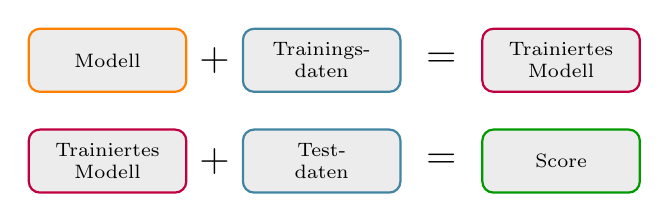
\begin{tikzpicture}[
    >=latex,
    font=\scriptsize,
    scale=0.8
]

% gemeinsame Breite
\def\w{2.0cm}

% obere Reihe
\node[draw=orange, thick, rounded corners, fill=gray!15,
      minimum width=\w, minimum height=0.8cm,
      align=center] at (0,1) {Modell};

\node[font=\Large\bfseries] at (1.7,1) {$+$};

\node[draw=cyan!60!black, thick, rounded corners, fill=gray!15,
      minimum width=\w, minimum height=0.8cm,
      align=center] at (3.4,1) {Trainings-\\daten};

\node[font=\Large\bfseries] at (5.3,1) {$=$};

\node[draw=purple, thick, rounded corners, fill=gray!15,
      minimum width=\w, minimum height=0.8cm,
      align=center] at (7.2,1) {Trainiertes\\Modell};

% untere Reihe
\node[draw=purple, thick, rounded corners, fill=gray!15,
      minimum width=\w, minimum height=0.8cm,
      align=center] at (0,-0.6) {Trainiertes\\Modell};

\node[font=\Large\bfseries] at (1.7,-0.6) {$+$};

\node[draw=cyan!60!black, thick, rounded corners, fill=gray!15,
      minimum width=\w, minimum height=0.8cm,
      align=center] at (3.4,-0.6) {Test-\\daten};

\node[font=\Large\bfseries] at (5.3,-0.6) {$=$};

\node[draw=green!60!black, thick, rounded corners, fill=gray!15,
      minimum width=\w, minimum height=0.8cm,
      align=center] at (7.2,-0.6) {Score};

\end{tikzpicture}

\column{0.45\textwidth}

\begin{itemize}
    \item Der erzielte \textbf{Score schwankt} abhängig von der Train/Test-Aufteilung.
    \item Die Schwankungen können reduziert werden, indem das Modell mit mehreren \textbf{unterschiedlichen Train/Test-Aufteilungen} trainiert und bewertet wird.
    \item Ein gängiges Verfahren hierfür ist die \textbf{k-fache Kreuzvalidierung}.
\end{itemize}

\end{columns}
\source{\cite{seemann2024mlaz}}
\end{frame}

\begin{frame}{k-fache Kreuzvalidierung}
\begin{columns}

\column{0.60\textwidth}

\centering
\begin{tikzpicture}[
    >=latex,
    font=\scriptsize,
    scale=0.8
]

% Achsen
\draw[TextColor, line width=1pt, ->] (0,0) -- (10,0);
\draw[TextColor, line width=1pt, ->] (0,0) -- (0,5);

% y-Achsenbeschriftung
\node[rotate=90, anchor=center, text=TextColor, font=\scriptsize\bfseries]
    at (-0.3,4.0) {Score};

% x-Ticks mit Beschriftung weiter links
\foreach \x/\i in {1/1,2/2,3/3,4/4,5/5,6/6,7/7,8/8}{
    \draw[TextColor] (\x,0) -- (\x,-0.2);
    \node[anchor=north east, rotate=90, text=DarkGrey]
        at (\x-0.3,-0.2) {\tiny Aufteilung \i};
}

% Horizontale Linie (Mittelwert)
\draw[PrimaryColor, line width=1.5pt] (0.2,2.8) -- (9.8,2.8);

% Punkte
\foreach \x/\y in {
    1/3.5,
    2/1.8,
    3/2.5,
    4/3.8,
    5/2.0,
    6/3.6,
    7/1.6,
    8/4.0
}{
    \node[draw=AccentTitle, very thick, cross out,
          minimum size=4pt, inner sep=0pt] at (\x,\y) {};
}

\end{tikzpicture}

\column{0.35\textwidth}

Der erzielte Score schwankt abhängig von der Train/Test-Aufteilung.

\vspace{0.4em}

Die Punkte zeigen die Ergebnisse für verschiedene Aufteilungen.

\vspace{0.4em}

Die Linie entspricht einem typischen \textbf{Mittelwert}.

\end{columns}
\source{\cite{seemann2024mlaz}}
\end{frame}

\begin{frame}{k-fache Kreuzvalidierung}
\begin{columns}

\column{0.35\textwidth}

\textbf{Vorgehen:}
\footnotesize   
\begin{itemize}
    \item Daten werden in $k$ Blöcke aufgeteilt
    \item Modell wird $k$-mal trainiert und bewertet
    \item Jeder Block wird \textbf{einmal als Testdaten} verwendet
    \item Restliche $k-1$ Blöcke sind Trainingsdaten
    \item \textbf{Ergebnis:} $k$ Scores
    \item Mittelwert der Scores als Gesamtbewertung
\end{itemize}

\column{0.60\textwidth}

\centering
\begin{tikzpicture}[
    scale=0.8,
    font=\scriptsize
]

% Breite
\def\w{1.3}

% Grundblock (grau)
\foreach \y in {0,1,2,3}{
    \draw[fill=gray!30] (0,\y*0.8) rectangle (\w,{\y*0.8+0.8});
}

% Fold 1
\foreach \y in {0,1,2,3}{
    \draw[fill=PrimaryColor!40] (2,\y*0.8) rectangle ({2+\w},{\y*0.8+0.8});
}
\draw[fill=AlertColor] (2,0) rectangle ({2+\w},0.8);
\node[text=white] at ({2+0.5*\w},0.4) {\tiny Test};

% Fold 2
\foreach \y in {0,1,2,3}{
    \draw[fill=PrimaryColor!40] (3.8,\y*0.8) rectangle ({3.8+\w},{\y*0.8+0.8});
}
\draw[fill=AlertColor] (3.8,0.8) rectangle ({3.8+\w},1.6);
\node[text=white] at ({3.8+0.5*\w},1.2) {\tiny Test};

% Fold 3
\foreach \y in {0,1,2,3}{
    \draw[fill=PrimaryColor!40] (5.6,\y*0.8) rectangle ({5.6+\w},{\y*0.8+0.8});
}
\draw[fill=AlertColor] (5.6,1.6) rectangle ({5.6+\w},2.4);
\node[text=white] at ({5.6+0.5*\w},2.0) {\tiny Test};

% Fold 4
\foreach \y in {0,1,2,3}{
    \draw[fill=PrimaryColor!40] (7.4,\y*0.8) rectangle ({7.4+\w},{\y*0.8+0.8});
}
\draw[fill=AlertColor] (7.4,2.4) rectangle ({7.4+\w},3.2);
\node[text=white] at ({7.4+0.5*\w},2.8) {\tiny Test};

% Scores
\node at (2.6,-0.6) {\small 0,85};
\node at (4.4,-0.6) {\small 0,95};
\node at (6.2,-0.6) {\small 0,88};
\node at (8.0,-0.6) {\small 0,92};
\node[font=\small\bfseries] at (1.0,-0.6) {Score:};

% Beschriftung links
\node[rotate=90, font=\small] at (-0.7,1.6) {Verfügbare Datensätze};

\end{tikzpicture}

\end{columns}
\source{\cite{seemann2024mlaz}}
\end{frame}

\makequizpage{\QUIZURL}{\QUIZQRCODE}{\QUIZIMAGE}

\begin{frame}[fragile]{k-fache Kreuzvalidierung in Python}
\begin{columns}

\column{0.35\textwidth}
\footnotesize
\textbf{Idee:}
\begin{itemize}
    \item Aufteilung der Daten in $k$ Blöcke
    \item \texttt{n\_splits} entspricht $k$
    \item \texttt{split()} liefert Indizes für:
    \begin{itemize}
        \item Trainingsdaten
        \item Testdaten
    \end{itemize}
\end{itemize}

\vspace{0.4em}
\textbf{Ablauf:}
\begin{enumerate}
    \item Aufteilung erzeugen
    \item Modell trainieren
    \item Modell bewerten
    \item Scores sammeln
\end{enumerate}

\column{0.60\textwidth}

\begin{minted}[fontsize=\footnotesize]{python}
from sklearn.model_selection import KFold

cv = KFold(n_splits=5) #k = 5
scores = []

for index_train, index_test in cv.split(X):
    # Daten aufteilen
    X_train = X[index_train]
    X_test = X[index_test]
    y_train = Y[index_train]
    y_test = Y[index_test]

    # Modell trainieren
    model = LinearRegression()
    model.fit(X_train, y_train)
    scores.append(model.score(X_test, y_test))
\end{minted}

\end{columns}
\source{\cite{seemann2024mlaz}, Kreuzvalidierung.ipynb}
\end{frame}

\begin{frame}[fragile]{k-fache Kreuzvalidierung in Python}
\footnotesize
\begin{columns}

\column{0.3\textwidth}

\textbf{Vereinfachung:}
\begin{itemize}
    \item Nutzung der Funktion \texttt{cross\_val\_score()}
    \item Übergabe von:
    \begin{itemize}
        \item Lernmodell
        \item Daten ($X$, $Y$)
        \item Kreuzvalidierungsstrategie (\texttt{cv})
    \end{itemize}
\end{itemize}

\vspace{0.4em}

\textbf{Ergebnis:}
\begin{itemize}
    \item Liste mit $k$ Scores
    \item Mittelwert als Gesamtbewertung
\end{itemize}

\column{0.65\textwidth}

\begin{minted}[fontsize=\footnotesize]{python}
from sklearn.model_selection import cross_val_score
from sklearn.model_selection import KFold

# 10-fache Kreuzvalidierung
kf = KFold(n_splits=10, shuffle=True)

# Scores berechnen
scores = cross_val_score(
    LinearRegression(), X, Y, cv=kf
)
print(scores)
print(np.mean(scores))
\end{minted}

\begin{minted}[fontsize=\footnotesize]{text}
[0.62853525 0.70270025 0.70362305 0.72788373 0.74651155 
0.64570138 0.78143471 0.71121285 0.67961735 0.65025846]
0.6977478575687336
\end{minted}

\end{columns}
\source{\cite{seemann2024mlaz}, KreuzvalidierungCrossValScore.ipynb}
\end{frame}


\begin{frame}{Übung: Kreuzvalidierung mit Diamanten}
\begin{columns}

\column{0.60\textwidth}
\footnotesize
Die Datei \texttt{diamonds.csv} enthält Daten zu mehr als 54\,000 Diamanten und deren Verkaufspreise.

\medskip

\textbf{Aufgaben:}
\begin{itemize}
\item Erstellen Sie zwei Modelle zur Vorhersage des Preises

\item \textbf{Modell A:} Preis nur anhand der Karat-Zahl (\texttt{carat})

\item \textbf{Modell B:} Preis anhand der Abmessungen (\texttt{x}, \texttt{y}, \texttt{z})

\item Bestimmen Sie das Bestimmtheitsmaß $R^2$ beider Modelle

\item Verwenden Sie eine \textbf{10-fache Kreuzvalidierung}

\item Mischen Sie die Daten vor der Kreuzvalidierung

\item Vergleichen Sie die Ergebnisse:
\begin{itemize}
    \item \footnotesize Welches Modell ist besser?
\end{itemize}
\end{itemize}

\column{0.35\textwidth}

\twemoji[width=0.9\linewidth]{laptop}

\end{columns}
\source{Lösung: LösungDiamanten.ipynb}
\end{frame}

\makequizpage{\QUIZURL}{\QUIZQRCODE}{\QUIZIMAGE}
\makequestionspage{\FRAGENIMAGE}